\documentclass{beamer}

\usepackage[T2A]{fontenc}
\usepackage[utf8]{inputenc}
\usepackage[russian]{babel}

\usetheme{Madrid}
\usecolortheme{whale}

\hypersetup {
    unicode = true
}

\title[Анализ подходов и средств]
{Анализ подходов и средств для верификации программ.
Использование фреймворков как средств автоматизации.}
\author[А.М. Полоцев]{
    А.М. Полоцев гр. 63501/13\\
    Современные проблемы информатики и вычислительной техники
}
\date[11.11.2013]{}

\begin{document}

\frame{\titlepage}

\begin{frame}
\frametitle{Основные понятия}

\textbf{Качество программного обеспечения} - это совокупность характеристик ПО,
относящихся к его способности удовлетворять установленные и предполагаемые
потребности.

\vspace{0.4cm}

\textbf{Верификация} проверяет соответствие одних создаваемых в ходе разработки
и сопровождения ПО артефактов другим, ранее созданным или используемым в
качестве исходных данных, а также соответствие этих артефактов и процессов их
разработки правилам и стандартам.

\vspace{0.4cm}

\textbf{Валидация} проверяет соответствие любых создаваемых или используемых в
ходе разработки и сопровождения ПО артефактов нуждам и потребностям
пользователей и заказчиков этого ПО, с учетом законов предметной области и
ограничений контекста использования ПО.

\end{frame}

\begin{frame}
\frametitle{Актуальность проблемы}

Сложность систем растет, сроки выпуска продуктов уменьшаются $\Rightarrow$
качество падает.

\vspace{0.4cm}

\tiny{\textit{Здесь должны быть примеры про падающие самолеты, облучение людей и т.д.}}

\centering {
\includegraphics[width=0.6\textwidth]{img/panic.png}
}

\end{frame}

\begin{frame}
\frametitle{Методы обеспечения качества}

\centering{
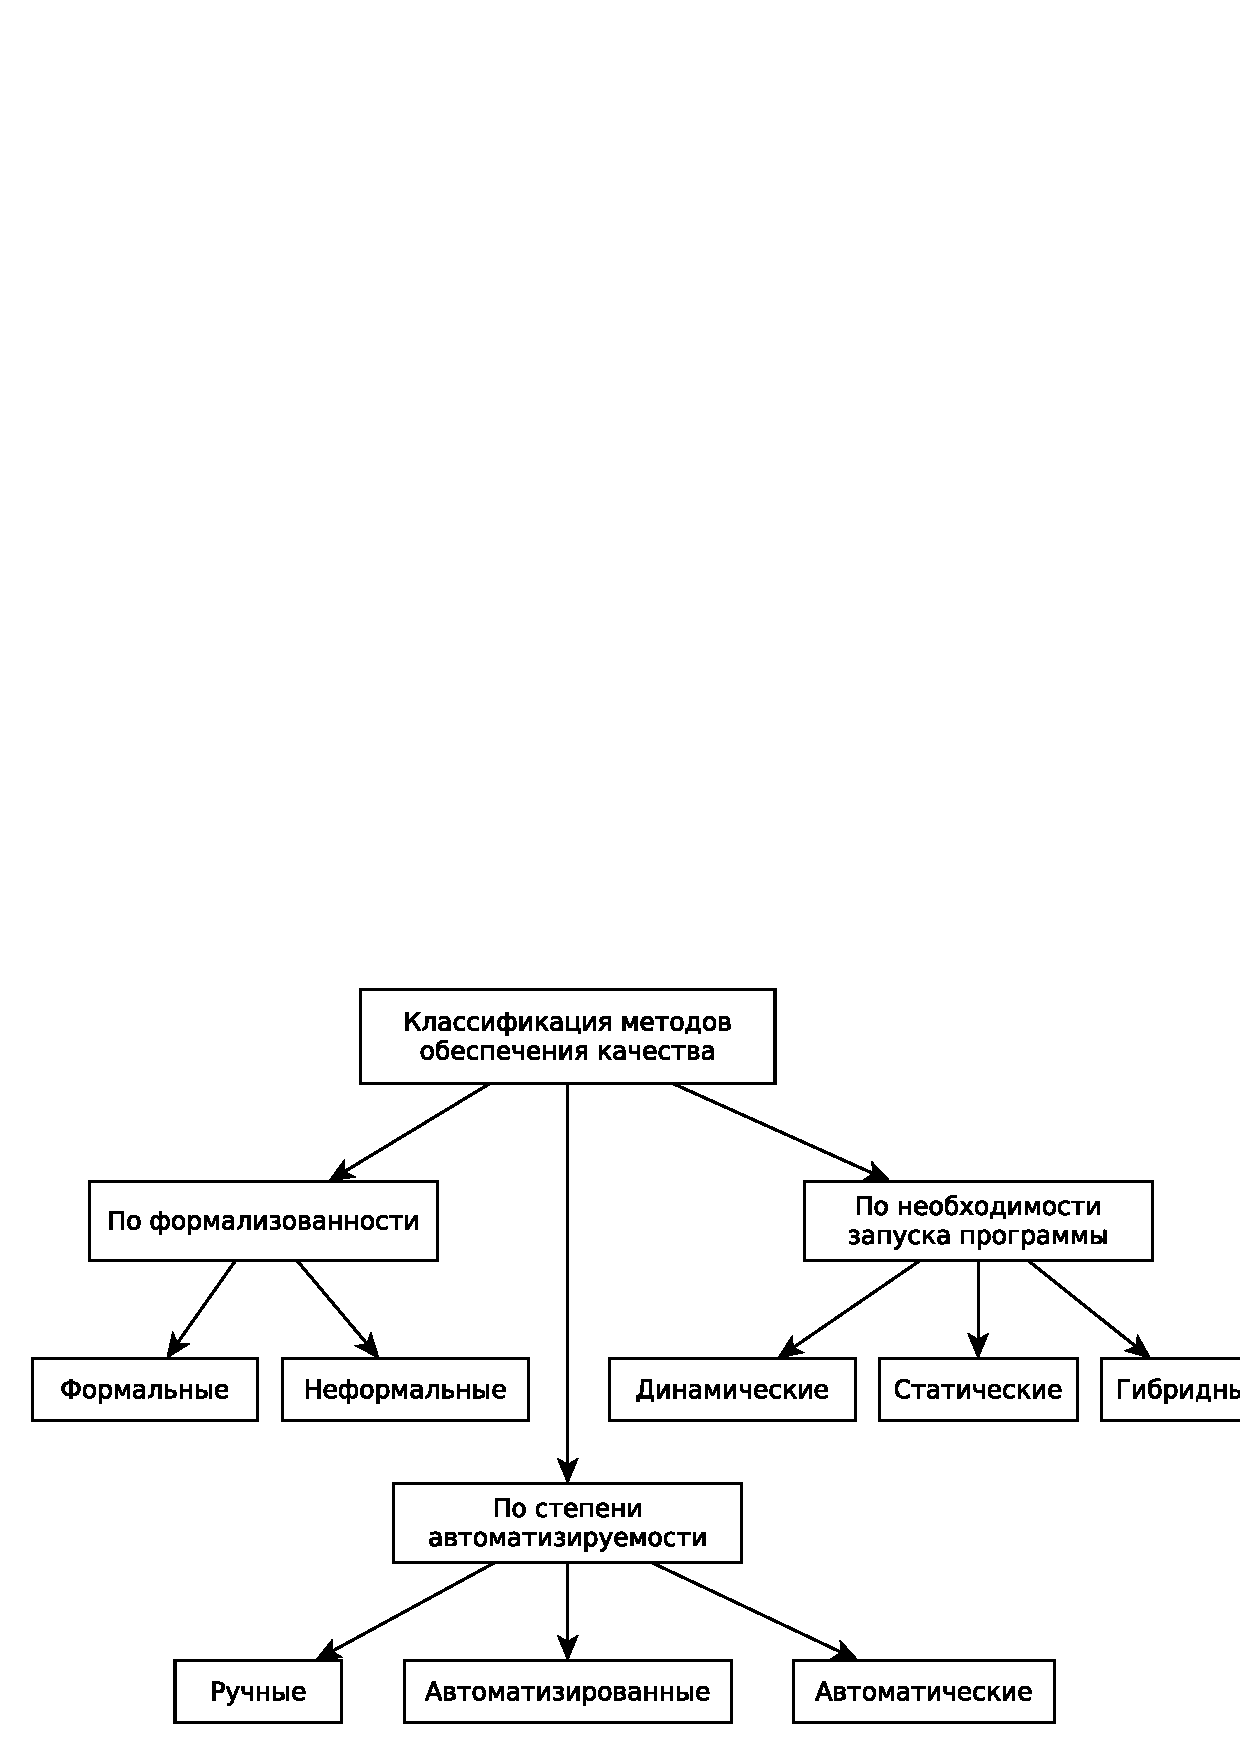
\includegraphics[width=0.8\textwidth]{img/verification_classification.png}
}

\end{frame}

\begin{frame}
\frametitle{Типичные задачи}

При проведении анализа ПО часто возникают следующие задачи:

\begin{enumerate}
    \item Построение моделей
    \begin{itemize}
        \item Абстрактное синтаксическое дерево
        \item Граф потока управления
        \item Граф зависимостей по данным
        \item Граф программных зависимостей
        \item Абстрактный семантический граф
        \item Статическое однократное присваивание
        \item ...
    \end{itemize}

    \item Построение метрик
    \begin{itemize}
        \item Метрики Холстеда
        \item Метрики Константейна и Йордана
        \item Метрики Отта и Мехра
        \item Метрики Абреу
        \item LOC
        \item ...
    \end{itemize}
\end{enumerate}

\end{frame}

\begin{frame}
\frametitle{Использование фреймворков для анализа ПО}

Для автоматизации анализа сложного ПО используются специализированные
инструментальные средства - фреймворки.

Решаемые задачи:

\begin{itemize}
    \item Построение метрик.
    \item Построение моделей программ и применение различных алгоритмов над
    этими моделями.
    \item Интерактивная визуализация процесса анализа.
\end{itemize}

\end{frame}

\begin{frame}
\frametitle{Упрощенная структура фреймворка}

\centering{
\includegraphics[width=\textwidth]{img/framework_structure.png}
}

\end{frame}

\begin{frame}
\frametitle{SMILE}

\begin{itemize}
    \item Фреймворк для построения метрик.
    \item В качестве метамодели используется eCST (enriched Concrete Syntax Tree).
    \item Находится в стадии разработки.
\end{itemize}

\end{frame}

\begin{frame}
\frametitle{SMILE}

\centering{
\includegraphics[width=0.7\textwidth]{img/smile_arch.png}
}

\end{frame}

\begin{frame}
\frametitle{Moose}

Moose является платформой для анализа программ и поддерживает большое количество
различных видов анализа:

\begin{enumerate}
    \item Построение и визуализация метрик.
    \item Обнаружение клонов.
    \item Построение графа зависимостей между пакетами.
    \item Вывод словаря, используемого в проекте.
    \item Поддержка браузеров исходного кода.
\end{enumerate}

\end{frame}

\begin{frame}
\frametitle{Moose}

\centering {
\includegraphics[width=\textwidth]{img/moose_architecture.png}
}

\end{frame}

\begin{frame}
\frametitle{LLVM}

\textbf{LLVM (Low Level Virtual Machine)} - фреймворк для построения компиляторов,
предназначен для анализа и трансформации программ.

\vspace{0.4cm}

LLVM использует промежуточное представление, в основе которого лежит
представление в виде SSA. Промежуточное представление является набором
RISC-подобных команд и содержит дополнительную информацию более высокого уровня,
например информацию о типах.

\end{frame}

\begin{frame}
\frametitle{LLVM}

\centering {
\includegraphics[width=\textwidth]{img/llvm_arch.png}
}

\end{frame}

\begin{frame}
\frametitle{Требования к разрабатываемому фреймворку}

Требуется создать среду для анализа программ, удовлетворяющую следующим
требованиям:

\begin{enumerate}
    \item Предоставлять API на языке Java для проведения анализа, а именно для
    построения различных метрик и моделей.
    \item Иметь модульную структуру - позволять подключать пользовательские
    алгоритмы анализа.
    \item Отображать полученные результаты в графическом виде.
\end{enumerate}

Все вышеперечисленные решения данным требованиям не удовлетворяют.

\pause

\begin{alertblock}{}
\centering{\Large{А это значит, что...}}
\end{alertblock}

\end{frame}

\begin{frame}
\frametitle{Hoist the code!}

\begin{block}{}
\centering{\Large{Нужно писать свой собственный!}}
\end{block}

\centering {
\includegraphics[width=0.6\textwidth]{img/pirate.jpg}
}

\end{frame}

\begin{frame}{Спасибо за внимание}
\center{\resizebox{60pt}{80pt}{?}}
\end{frame}

\end{document}
